\chapter{Design}

\section{Architecture}
Moving towards architecture, we first have to separate the whole system into smaller parts that share the same responsability. \\
This way, I can foresee four main services:
\begin{itemize}[noitemsep]
    \item \textbf{Auth/User service:} to manage authorization and authentication.
    \item \textbf{Stats service:} to manage all the information related to stats diagram generation. 
    \item \textbf{Test service:} to manage the test creation, indicate if a reply is correct or not...It should be able to generate the tests from the dataset and get the videos for the helper videos and to form the tests.
    \item \textbf{Video recognition service:} AI service to validate a video sent by the user. It will classify the video into labels.
\end{itemize}

There should be a direct communication between the \textit{Stats service} and the \textit{Test service} because the stats should be created from the data stored from the tests. \\
Also, there should be communication between the \textit{Video recognition service} and the \textit{Test service} because in order to update if a reply is okay or not, the {Test service} should know if the user signed correctly in some particular cases.

\begin{figure}[H]
    \centering
        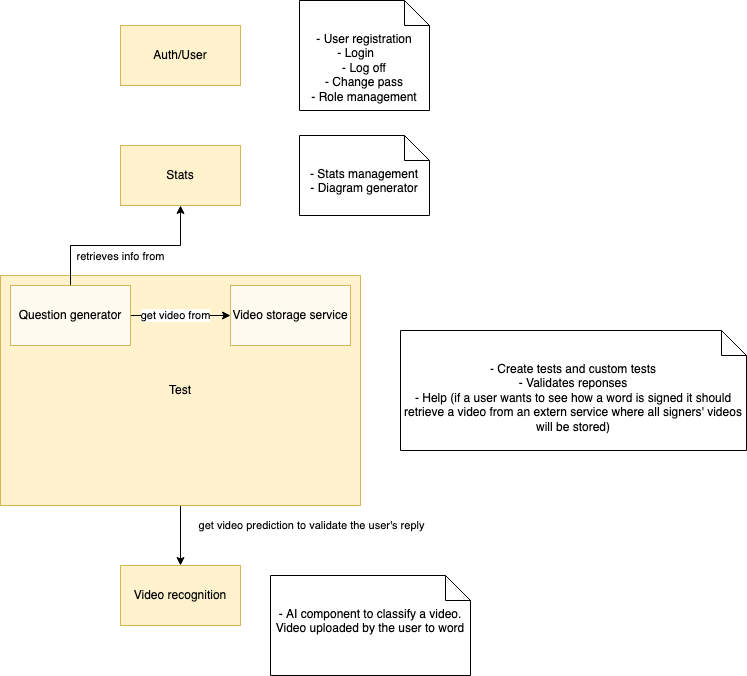
\includegraphics[width=\textwidth]{assets/diagrams/services.png}
    \caption{Towards the app's architecture}
    \label{fig:design_architecture_first}
\end{figure}

Reiterating the last diagram, I got this one, which specifies better the entities. The user communicates with the app, which is formed by the four subsystems. I can have two databases, one for user identification (\textbf{Auth}) and another one for user stats, info about the tests done by them...(\textbf{User stats}). \\

The main difference now is the communication part: the \textit{stats service} does not need to communicate with the \textit{test service}, as the stats can be dynamically created from the info of the database. 

\begin{figure}[H]
    \centering
        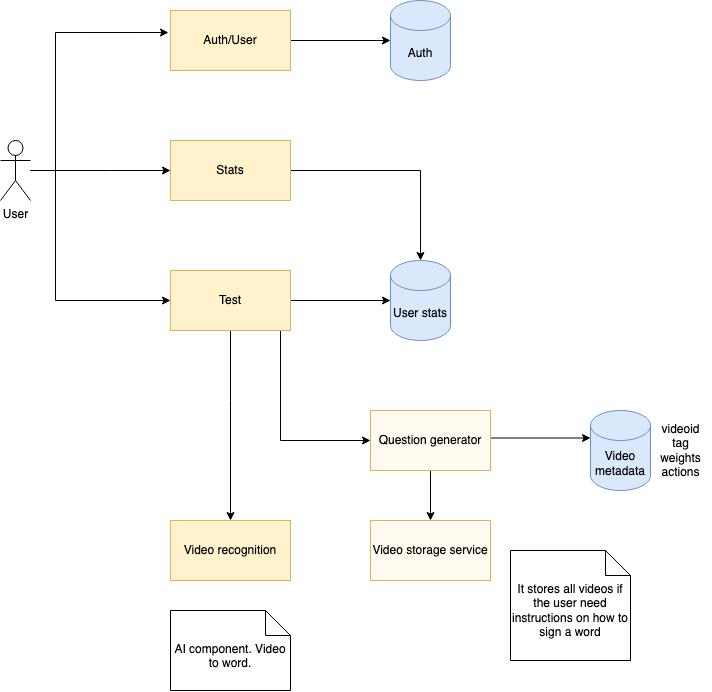
\includegraphics[width=\textwidth]{assets/diagrams/architecture.png}
    \caption{App's architecture}
    \label{fig:design_architecture_last}
\end{figure}

\section{Conceptual design}
As I finally came to understand the better the entities of the application and their relationship, I created a new diagram to simplify all of them. \\

By doing this diagram, I got clearer that the event that changed the stats was the case when a user does a test. Also, I got a new entity: \textit{Question}, which is the base component to form a test. The question comes from the \textit{question generator}, that using the \textit{video storage service} (which can be an extern service) and the \textit{dataset} creates the questions.

\begin{figure}[H]
    \centering
        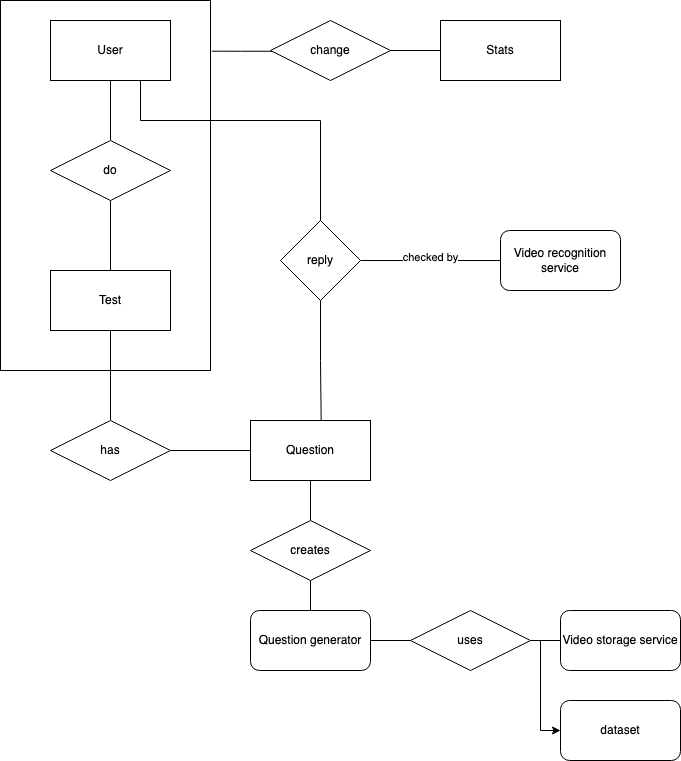
\includegraphics[width=\textwidth]{assets/diagrams/conceptual.png}
    \caption{App's architecture}
    \label{fig:design_conceptual}
\end{figure}

\section{UI design}
\subsection{Low fidelity design}
To validate all the features that the application should have, the navigation, implementation of user stories, design patterns...I created a low-fidelity design. \\

Firstly, I present all the screens created drawing in a tablet. Then, I present the navigation between these screens, so that you can see the flow of the application and how \\
an user should interact with the app itself. \\

I used a mobile as the device as this is the minimum hardware neccessary to use the application and most users nowadays use mobile devices. \\
In order to launch a viable product, I should research the neccessities of these users and study their behaviour. This way, I could know if most of the users \\
wanted to use their pc, tablet instead of mobile devices or they had additional hardware such as external cameras or support devices so that they can use both hands with \\
their mobiles in order to sign correctly. As I don't have the resources and knowledge to do a really useful study of this kind, I selected the minimum device unit and \\
a type of product and tools that could then be migrated to any device (web technology using React could be used in any device and then be migrated to React Native or a PWA reusing most of the components).\\
\subsubsection{Common}
These are the commons components for the whole application. The \textbf{navbar} and the \textbf{bottom bar}. \\

The \textbf{navbar} shows basic information about the current user and allow a quick navigation to secondary info about the app. \\
It could have information about the current page, but this won't be neccessary as I apply the \textit{3-step rule} and there is no much information in this application. \\
What it is important about the navbar, it is that it will allow the navigation to the last page.

The \textbf{bottom bar} allow the user to navigate through the main pages of the application. It won't be visible in subpages to allow the user to concentrate in a task and \\
gain space in the screen. \\
\begin{figure}[H]
    \centering
    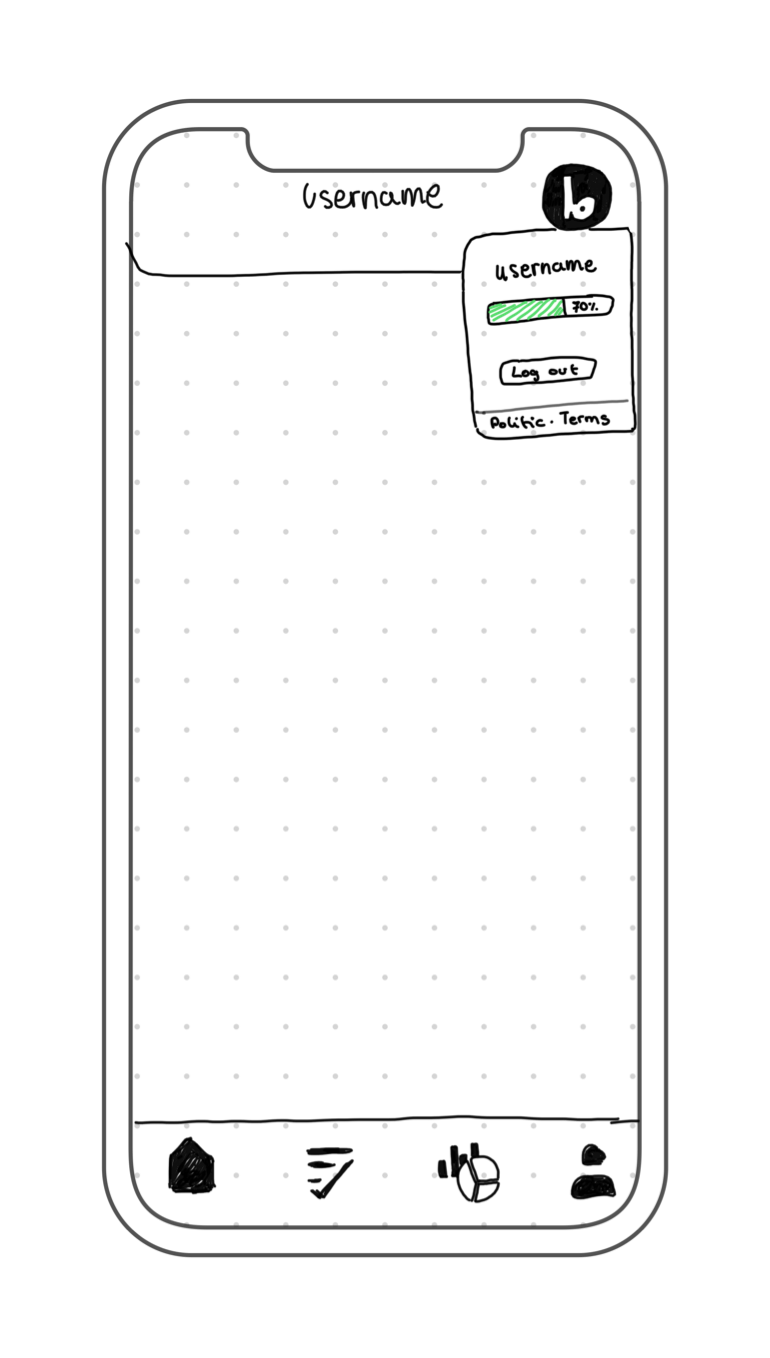
\includegraphics[width=0.24\textwidth]{assets/screens/Button - User.png}
    \caption{Common components}
    \label{fig:design_common}
\end{figure}

\subsubsection{Authorization}
These screens just show the initial pages of the application. In order to be used, being logged in is needed, so the user should be firstly registered and then signed in to start a new session.\\

orify: \textit{RF\_1.1} and \textit{RF\_1.2}. \\
\begin{figure}[H]
    \centering
    \begin{subfigure}[T]{0.49\textwidth}
        \centering
        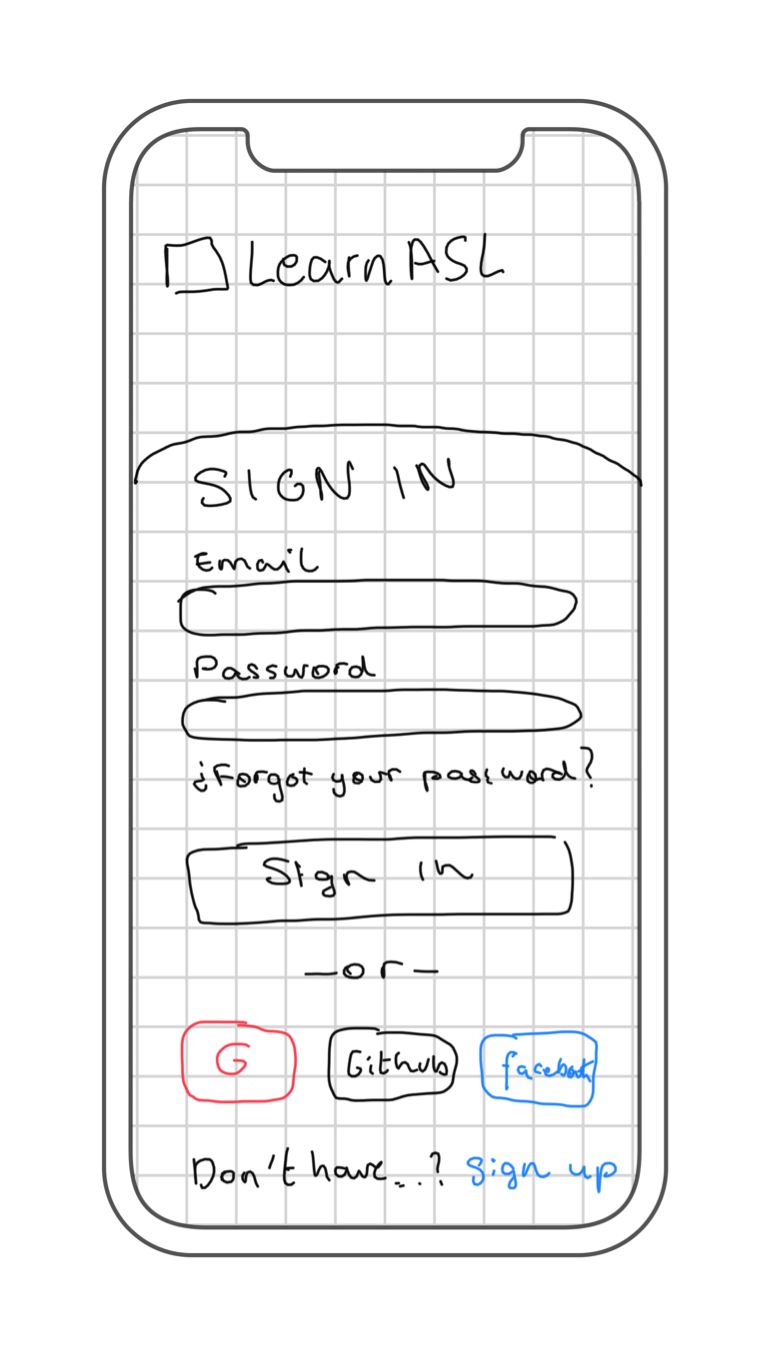
\includegraphics[width=0.48\textwidth]{assets/screens/auth/Login.png}
        \caption{Login screen}
        \label{fig:design_screen_login}
    \end{subfigure}
    \hfill
    \begin{subfigure}[T]{0.49\textwidth}
        \centering
        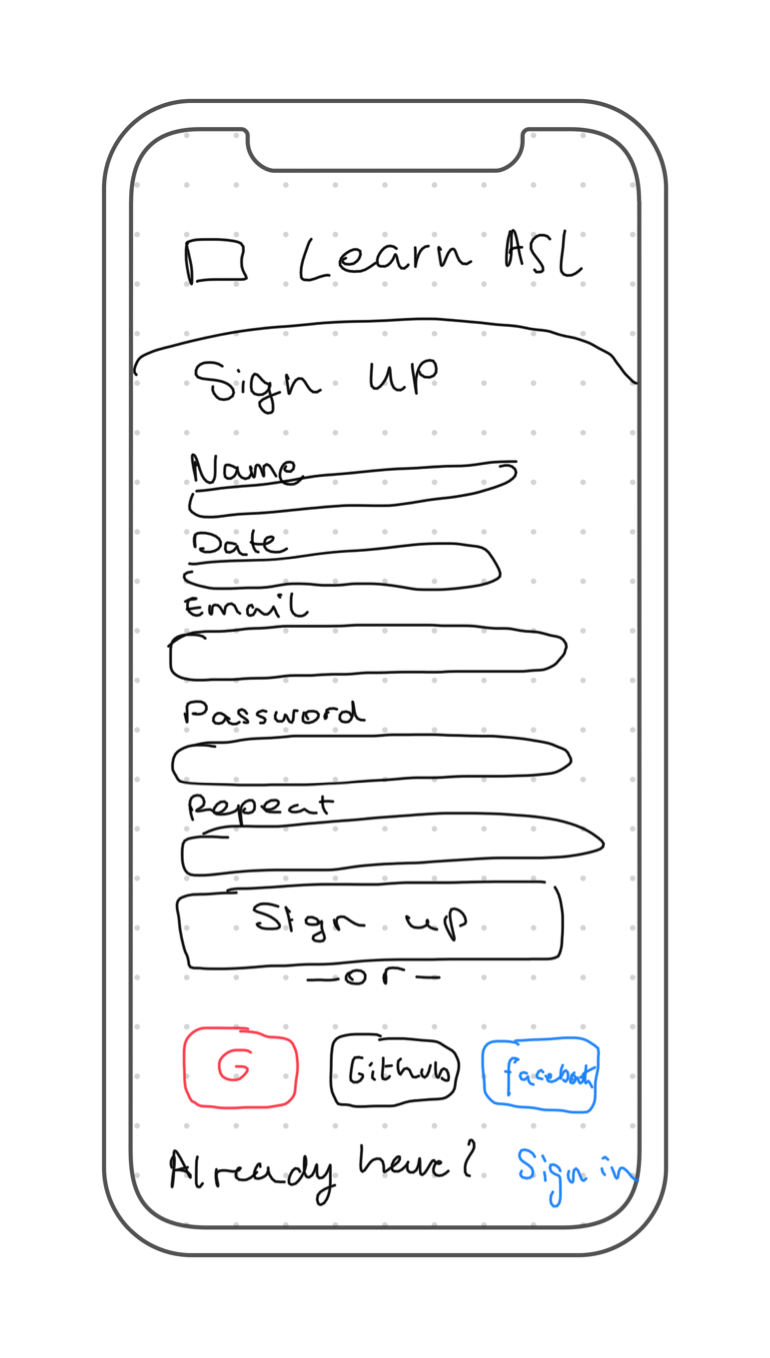
\includegraphics[width=0.48\textwidth]{assets/screens/auth/Register.png}
        \caption{Register screen}
        \label{fig:design_screen_camera_register}
    \end{subfigure}
       \caption{Authorization screens}
       \label{fig:design_screens_auth}
\end{figure}

\subsubsection{Home}
The home screen will show the main information a user want to access. This is the recent quizs taken by the user. \\

In addition, I included an \textbf{ad component}, so that the monetization model of the app could be via ads. This should be taken into account when the app is going to be launched in production and to create a valid business model.\\

It satifies: \textit{RF\_2.3}. \\
\begin{figure}[H]
    \centering
        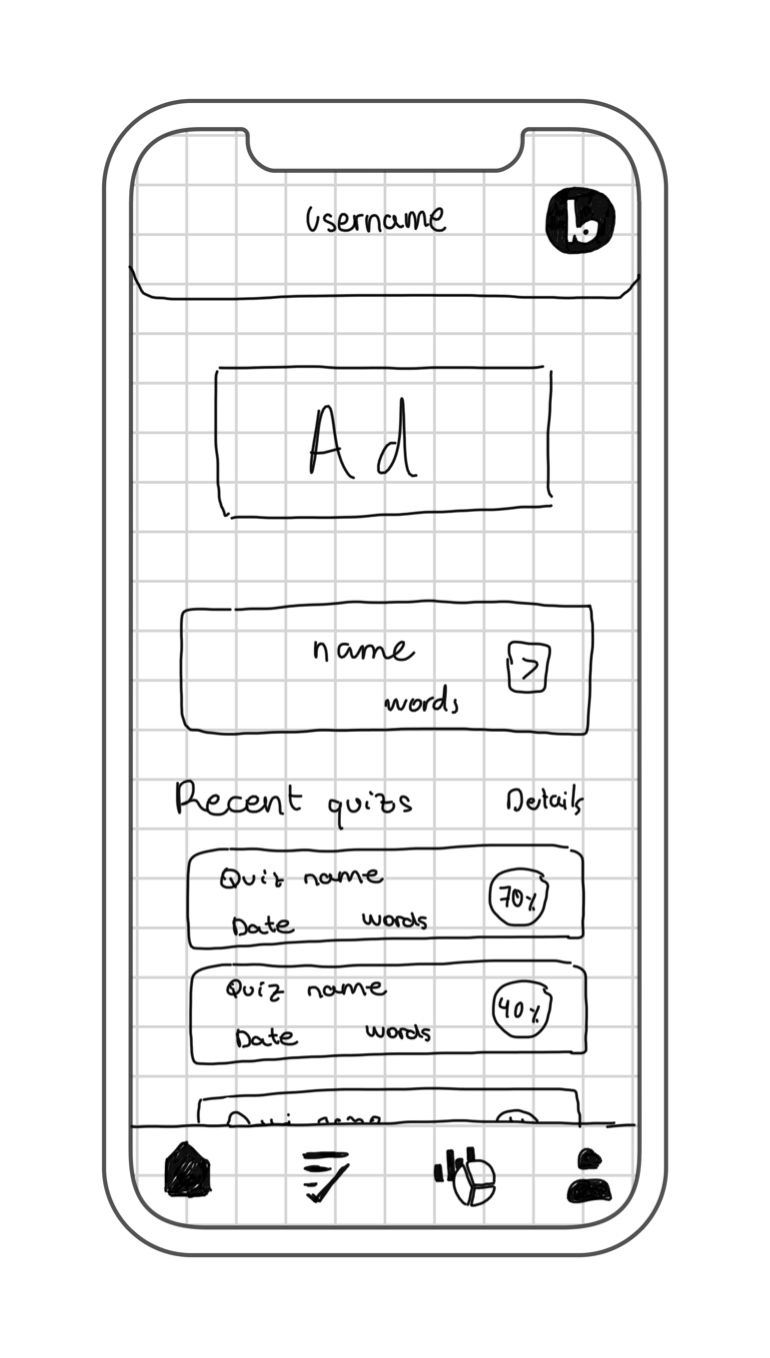
\includegraphics[width=0.24\textwidth]{assets/screens/Home.png}
    \caption{Home screen}
    \label{fig:design_home}
\end{figure}

\subsubsection{Quiz}
These are the common components/screens for the quizs. \\

Firstly, we see a \textbf{result screen}, in which the user can see how they performed doing the current quiz. This could be reusable when the user is reviewing an already done quiz. \\
As the main objective of an user in the application is to do quizes, it has a button to easily access this feature. \\
A share button is included so that the application can gain visibility via users. The main objective of this is not fomenting competitivity, but gaining visibility in social network platforms. \\

Secondly, we see a \textbf{selecting difficulty screen}. The user will be able to customize a quiz, selecting the \textbf{difficulty} and the \textbf{number of questions} of a test. \\

Finally, we see a \textbf{selecting quiz's type screen}. The user will be able to select the \textbf{test type} before starting a new one. \\
\begin{figure}[H]
    \centering
    \begin{subfigure}[T]{0.32\textwidth}
        \centering
        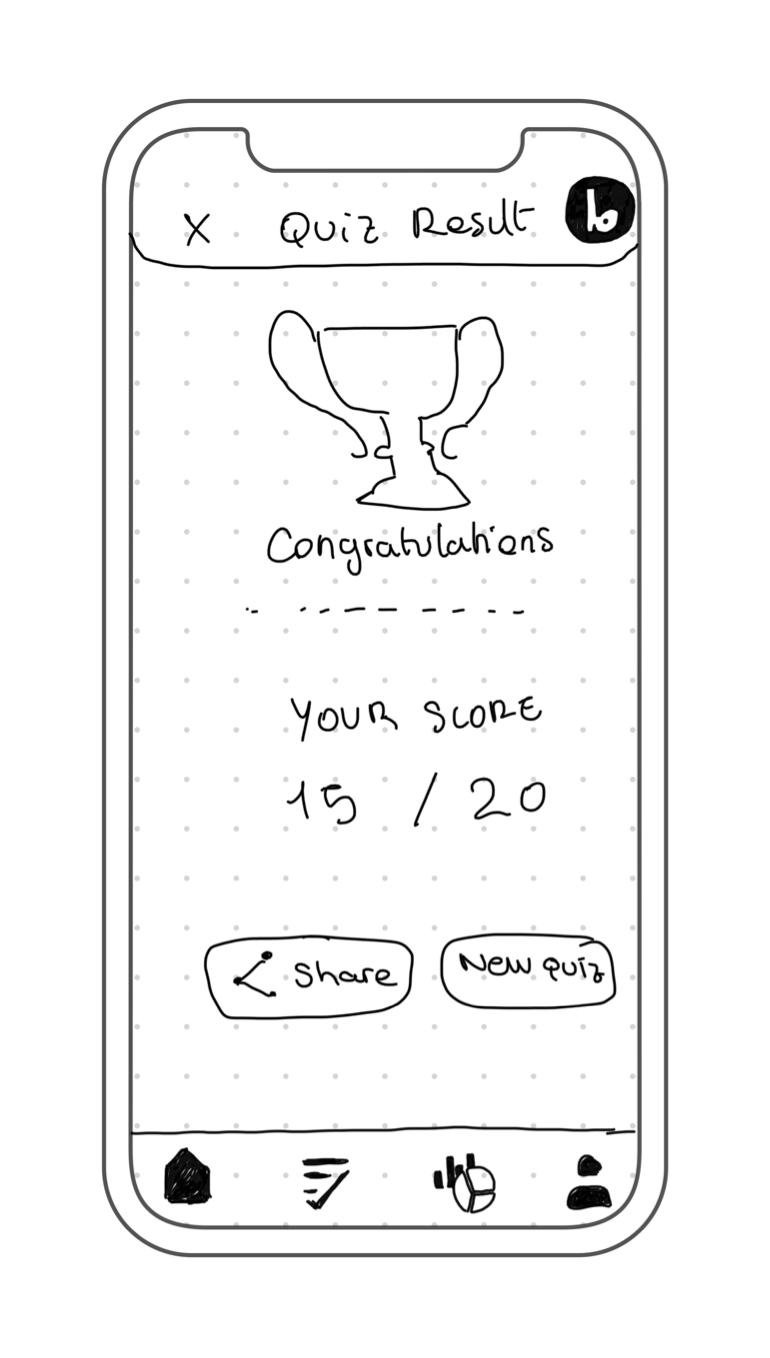
\includegraphics[width=0.72\textwidth]{assets/screens/quiz/common/Quiz - Result.png}
        \caption{Result of a test}
        \label{fig:design_screen_result}
    \end{subfigure}
    \hfill
    \begin{subfigure}[T]{0.33\textwidth}
        \centering
        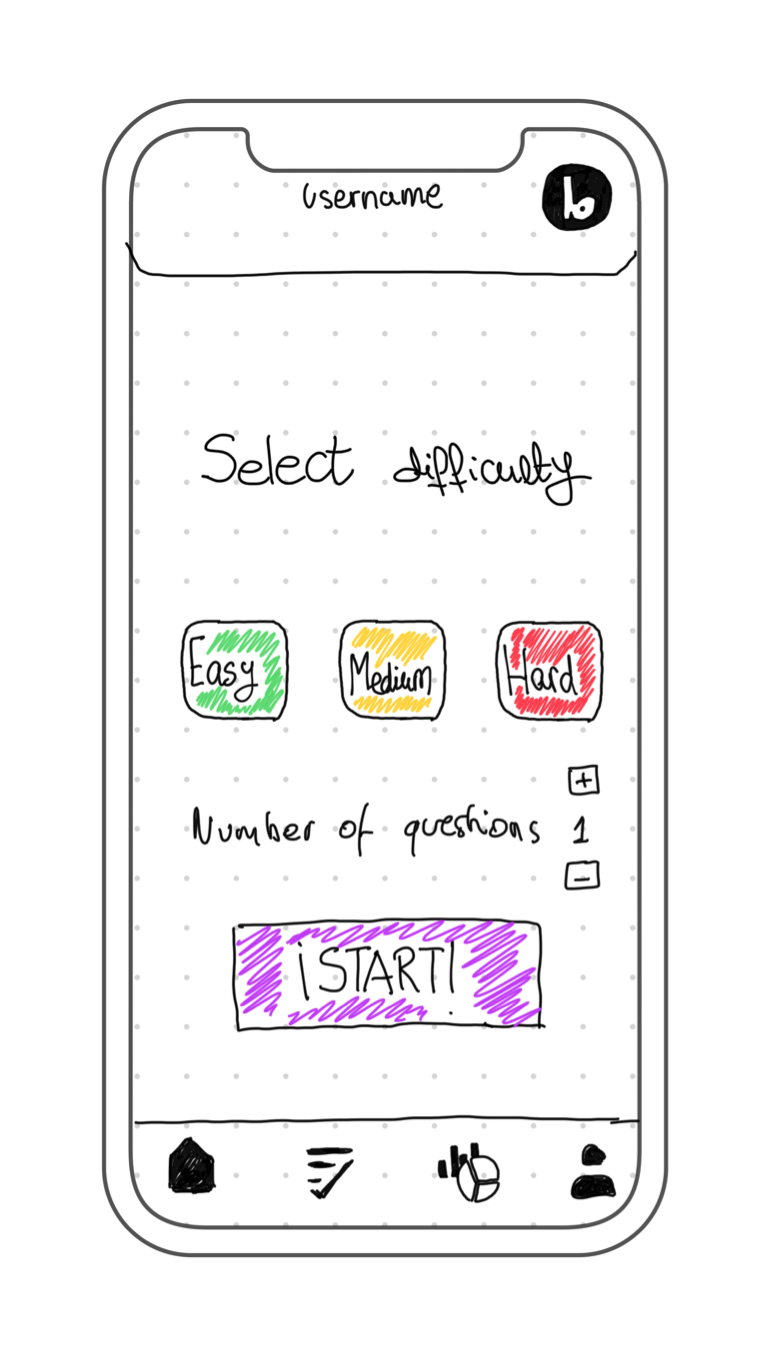
\includegraphics[width=0.72\textwidth]{assets/screens/quiz/common/Select difficulty.png}
        \caption{Select difficulty of a test}
        \label{fig:design_screen_select_dif}
    \end{subfigure}
    \hfill
    \begin{subfigure}[T]{0.33\textwidth}
        \centering
        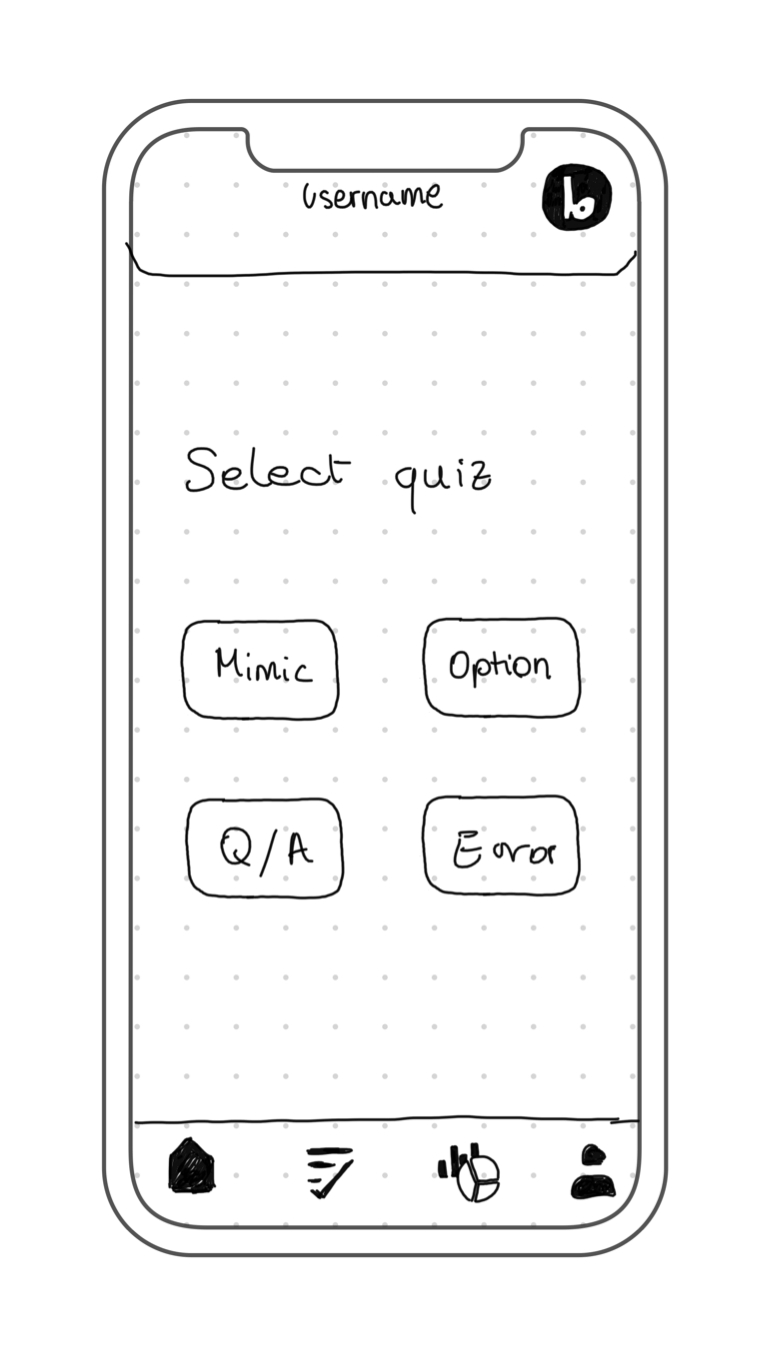
\includegraphics[width=0.72\textwidth]{assets/screens/quiz/common/Select quiz.png}
        \caption{Select type of test}
        \label{fig:design_screen_select_quiz}
    \end{subfigure}
       \caption{Common screens for all tests}
       \label{fig:design_test_common}
\end{figure}
Here I am presenting the quizes themselves. What it is important to notice is that the user can \textbf{skip} a question, see how many questions the current quiz has, the test type and a feedback for the question result, as well as the number of the current question. \\

\begin{itemize}[noitemsep]
    \item \textbf{Mimic:} the question is composed by the word to sign and a help video. The user should sign themselves signing that word and can watch the help video to imitate it.
    \item \textbf{Option video to word:} the question is composed by a video representing a sign and 4 options (words). The user should select the word matching the video.
    \item \textbf{Option word to video:} the question is composed by a word and 4 videos representing signs. The user should select the video that signs correctly the asked word.
    \item \textbf{QA:} the question is composed by just the word to sign. The user should sign the word.
\end{itemize}
\begin{figure}[H]
    \centering
    \begin{subfigure}[T]{0.24\textwidth}
        \centering
        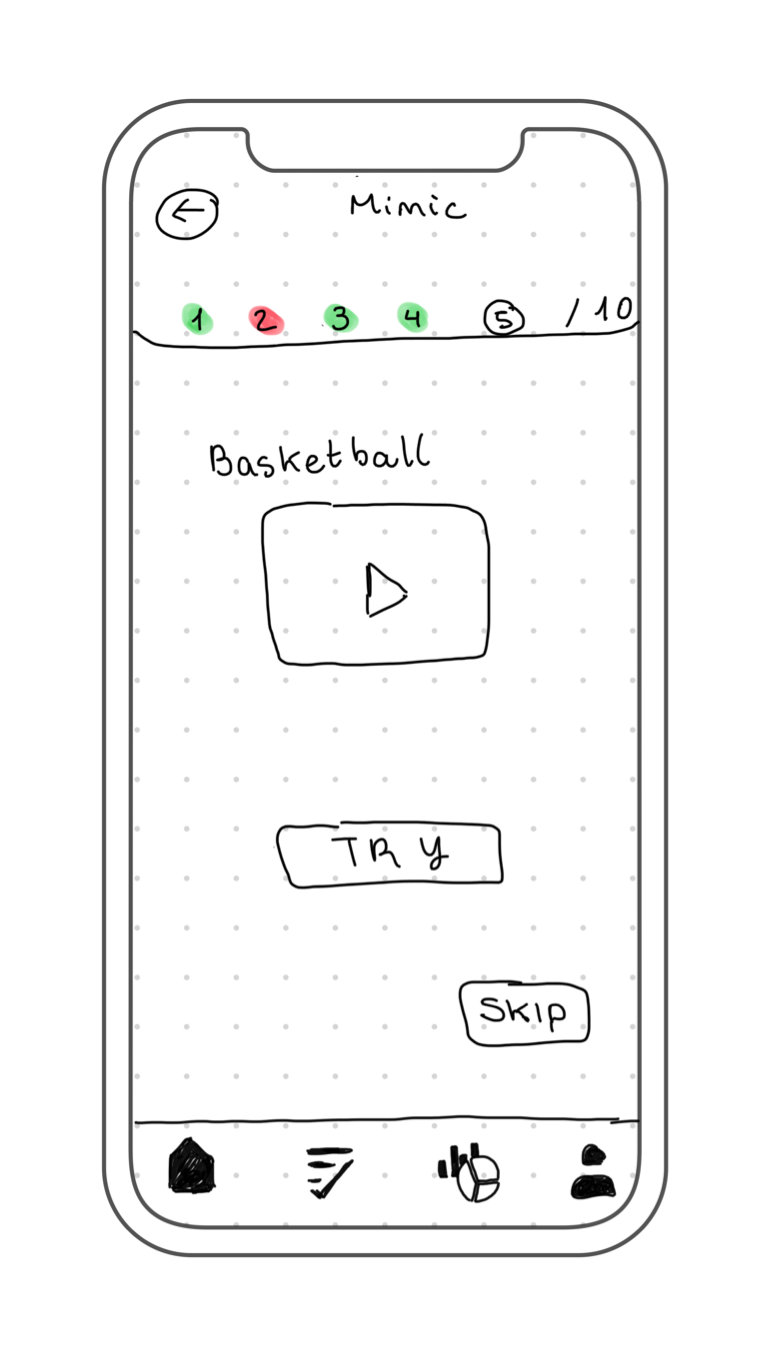
\includegraphics[width=\textwidth]{assets/screens/quiz/Quiz - Mimic.png}
        \caption{Mimic}
        \label{fig:design_screen_mimic}
    \end{subfigure}
    \hfill
    \begin{subfigure}[T]{0.24\textwidth}
        \centering
        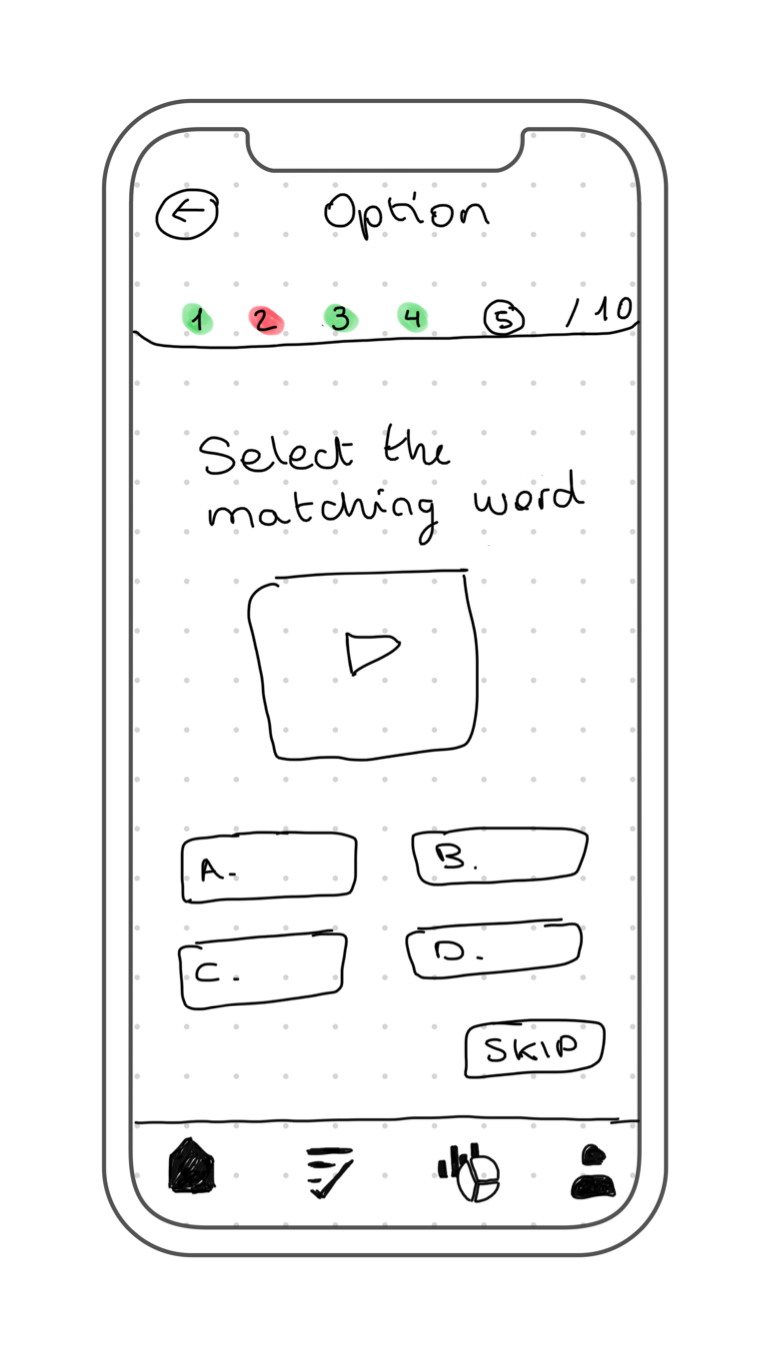
\includegraphics[width=\textwidth]{assets/screens/quiz/Quiz - Option 1.png}
        \caption{Option video to word}
        \label{fig:design_screen_mimic}
    \end{subfigure}
    \hfill
    \begin{subfigure}[T]{0.24\textwidth}
        \centering
        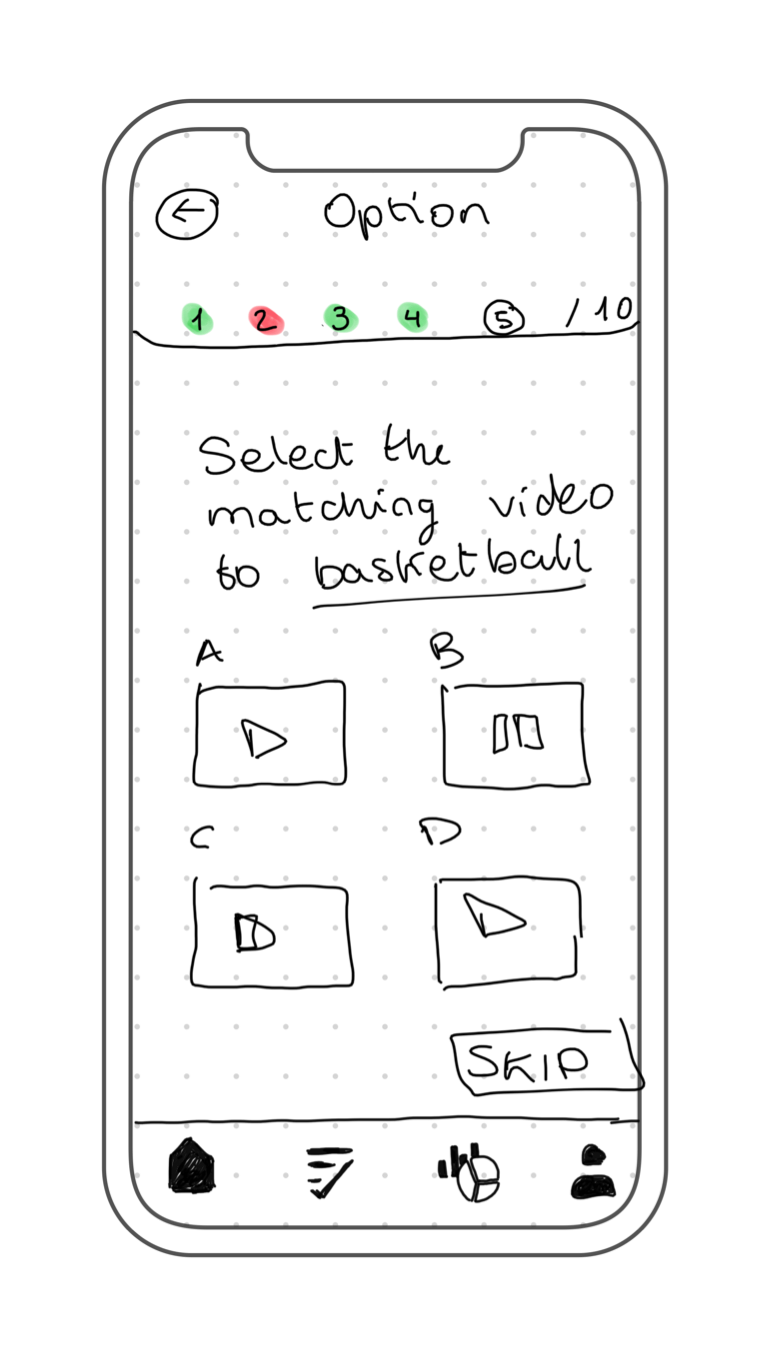
\includegraphics[width=\textwidth]{assets/screens/quiz/Quiz - Option 2.png}
        \caption{Option word to video}
        \label{fig:design_screen_mimic}
    \end{subfigure}
    \begin{subfigure}[T]{0.24\textwidth}
        \centering
        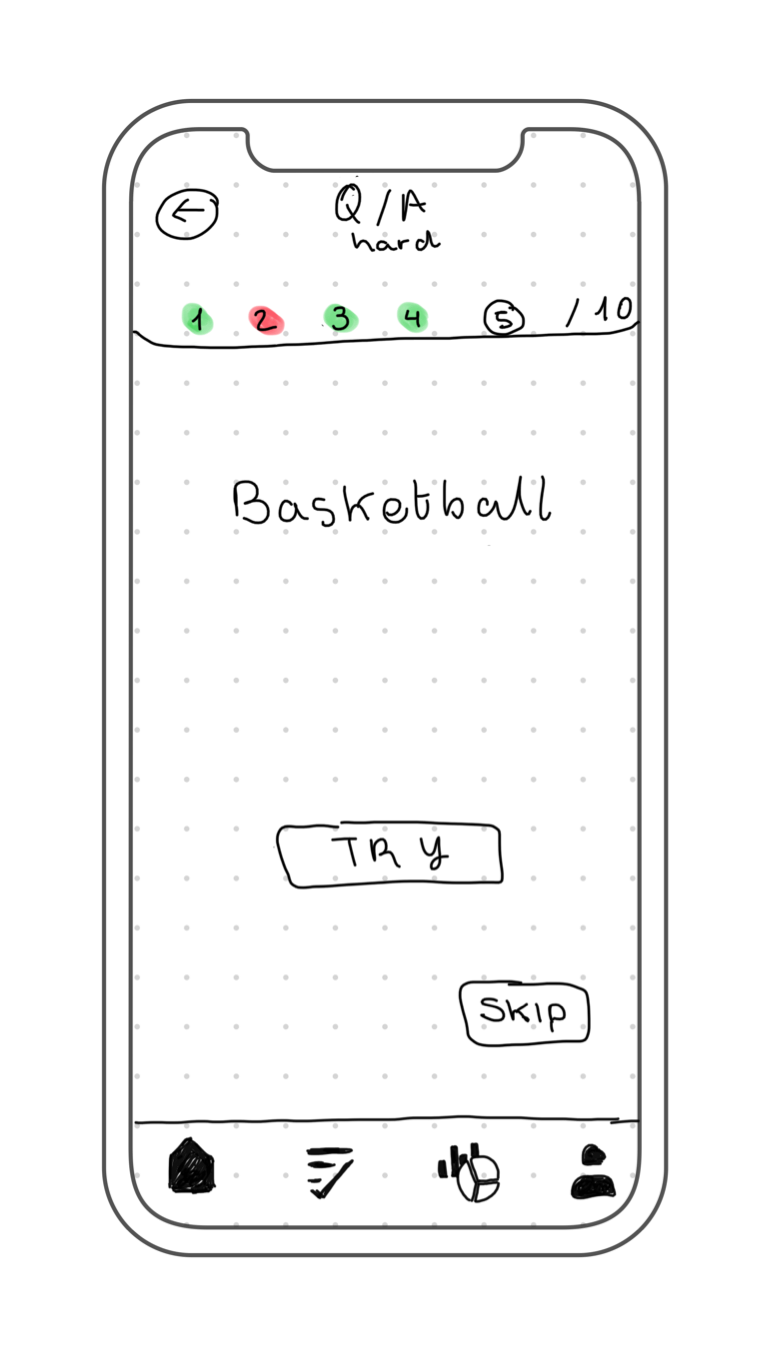
\includegraphics[width=\textwidth]{assets/screens/quiz/Quiz - Q_A.png}
        \caption{QA}
        \label{fig:design_screen_mimic}
    \end{subfigure}
       \caption{Tests' screens}
       \label{fig:design_test_screen}
\end{figure}

These screens represent how a user could reply to a question if they are asked to send a video. They could select a video from the gallery or record them signing the word, and send the video to the application or record it again. \\
\begin{figure}[H]
    \centering
    \begin{subfigure}[T]{0.49\textwidth}
        \centering
        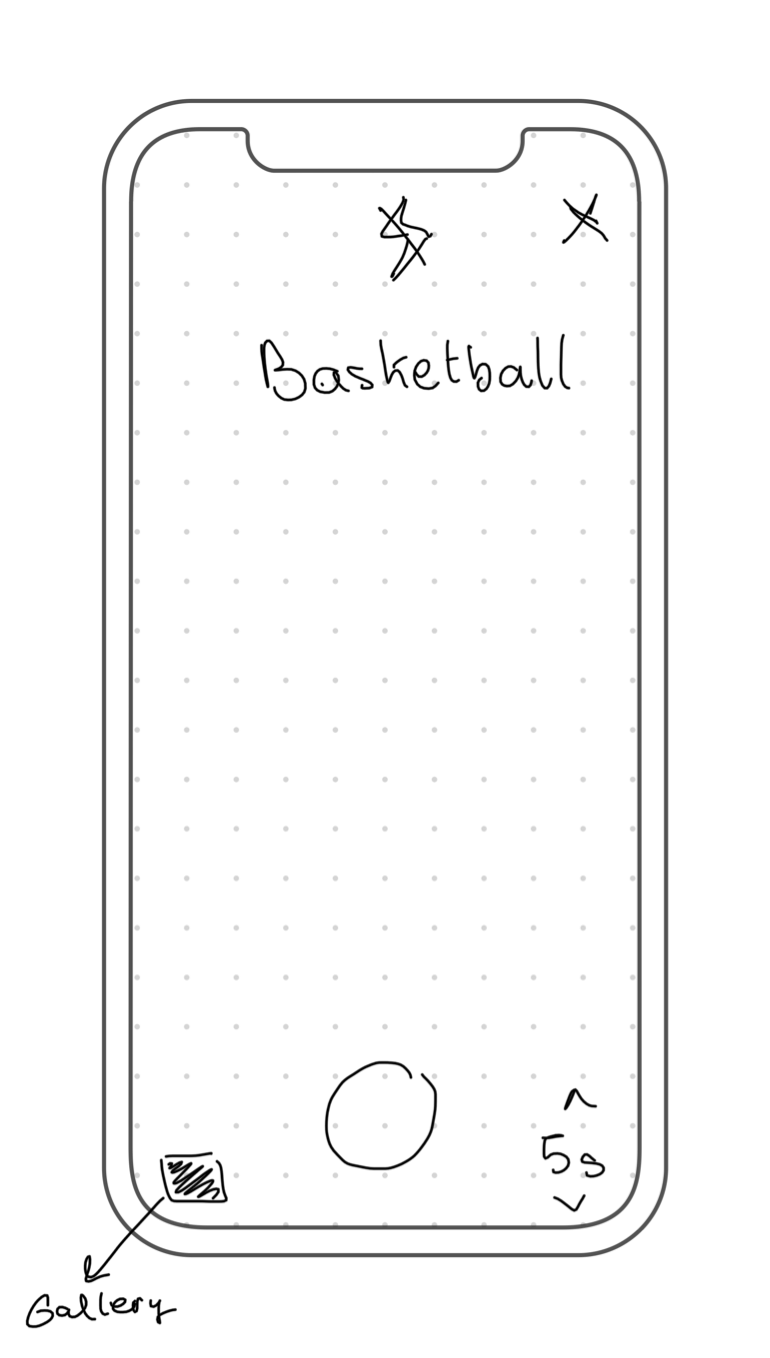
\includegraphics[width=0.48\textwidth]{assets/screens/quiz/quiz-camera/Quiz - Camera.png}
        \caption{Camera}
        \label{fig:design_screen_camera}
    \end{subfigure}
    \hfill
    \begin{subfigure}[T]{0.49\textwidth}
        \centering
        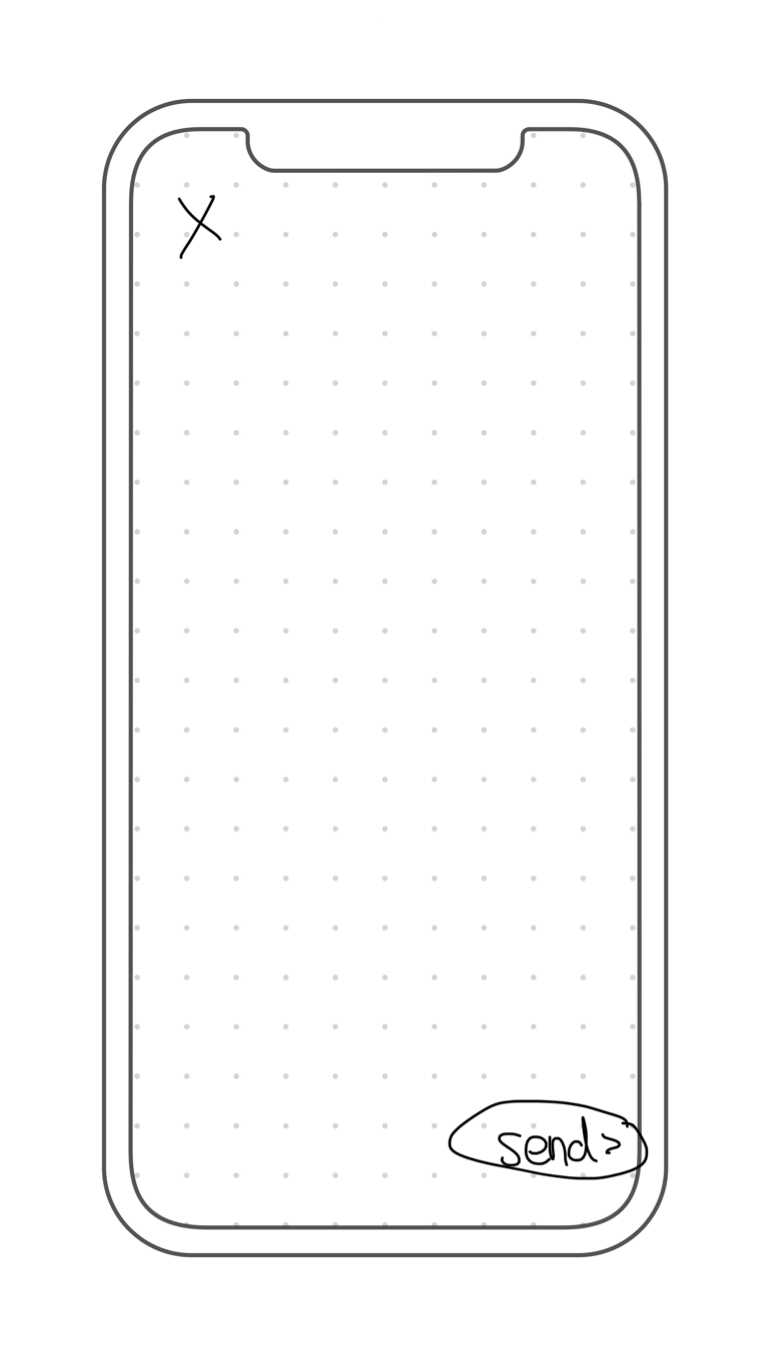
\includegraphics[width=0.48\textwidth]{assets/screens/quiz/quiz-camera/Quiz - Camera send.png}
        \caption{Send photo}
        \label{fig:design_screen_camera_send}
    \end{subfigure}
       \caption{Reply to test using the camera}
       \label{fig:design_camera}
\end{figure}

\subsubsection{Stats}
In order to show the stats to the user, a stat screen is added. \\

The first screen represent the most basic information: the \textbf{percent of learnt words} and the \textbf{use of the app} (in the calendar an user can see the days they have used the application starting a new quiz). They also can consult the maximum number of days they have used the application in a row and the current streak. \\

The second screen shows more information about the app to the user: \textbf{time spent} in the app and \textbf{new words learnt}, as well as the \textbf{success rate}. The users can filter the stats by date (and/or) by difficulty. \\

The third screen show another way of representing the stats, in a more detailed way using graphs. \\

orify: \textit{RF\_3.1} and \textit{RF\_3.2}. \\
\begin{figure}[H]
    \centering
    \begin{subfigure}[T]{0.32\textwidth}
        \centering
        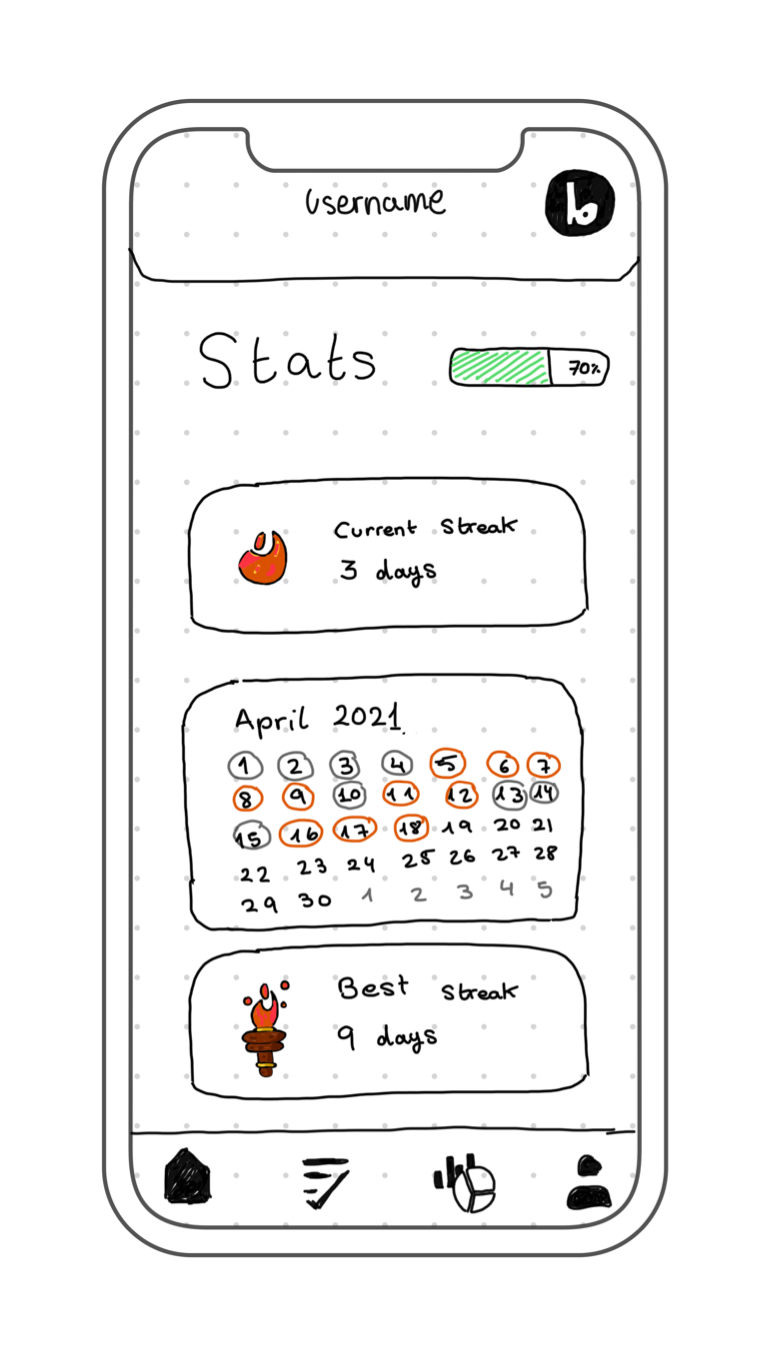
\includegraphics[width=0.72\textwidth]{assets/screens/stats/Stats - 1.png}
        \caption{Stats: page 1}
        \label{fig:design_screen_stats_1}
    \end{subfigure}
    \hfill
    \begin{subfigure}[T]{0.32\textwidth}
        \centering
        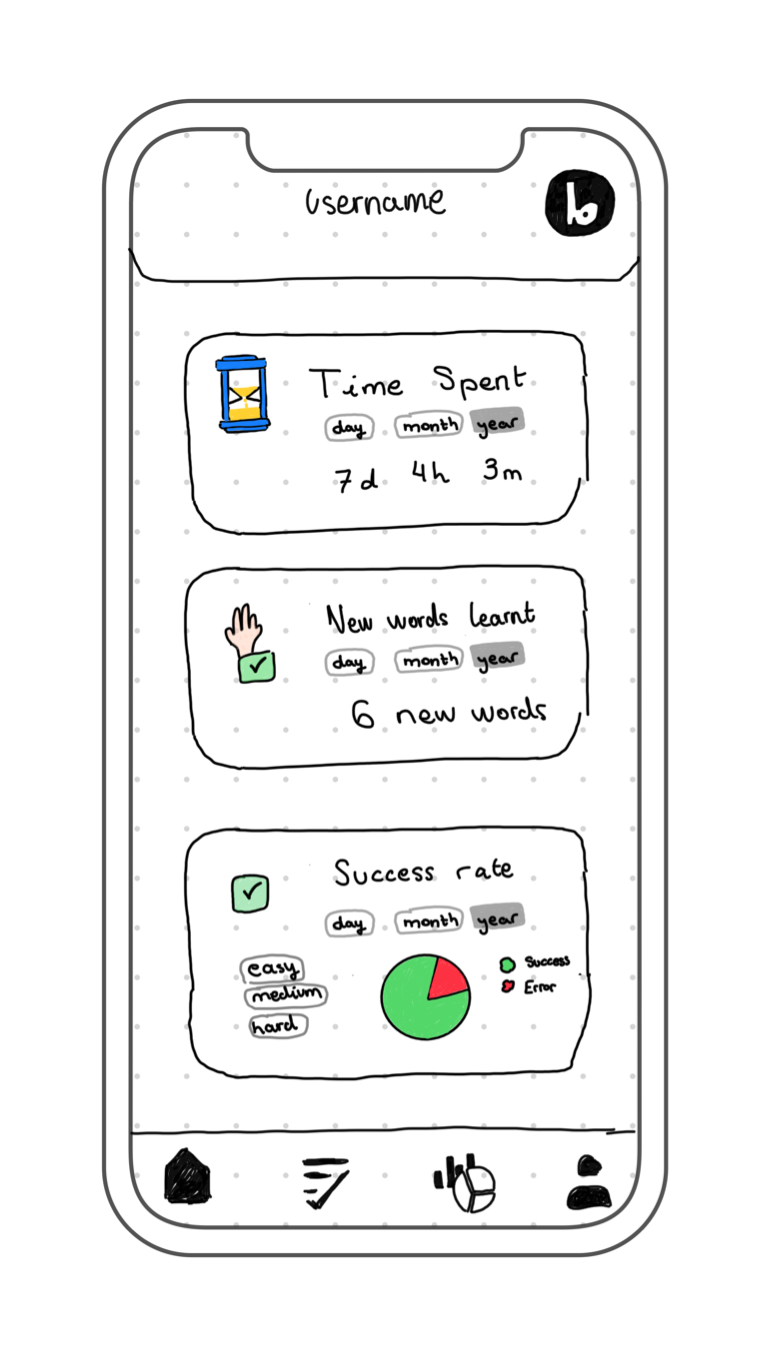
\includegraphics[width=0.72\textwidth]{assets/screens/stats/Stats - 2.png}
        \caption{Stats: page 2}
        \label{fig:design_screen_stats_2}
    \end{subfigure}
    \hfill
    \begin{subfigure}[T]{0.32\textwidth}
        \centering
        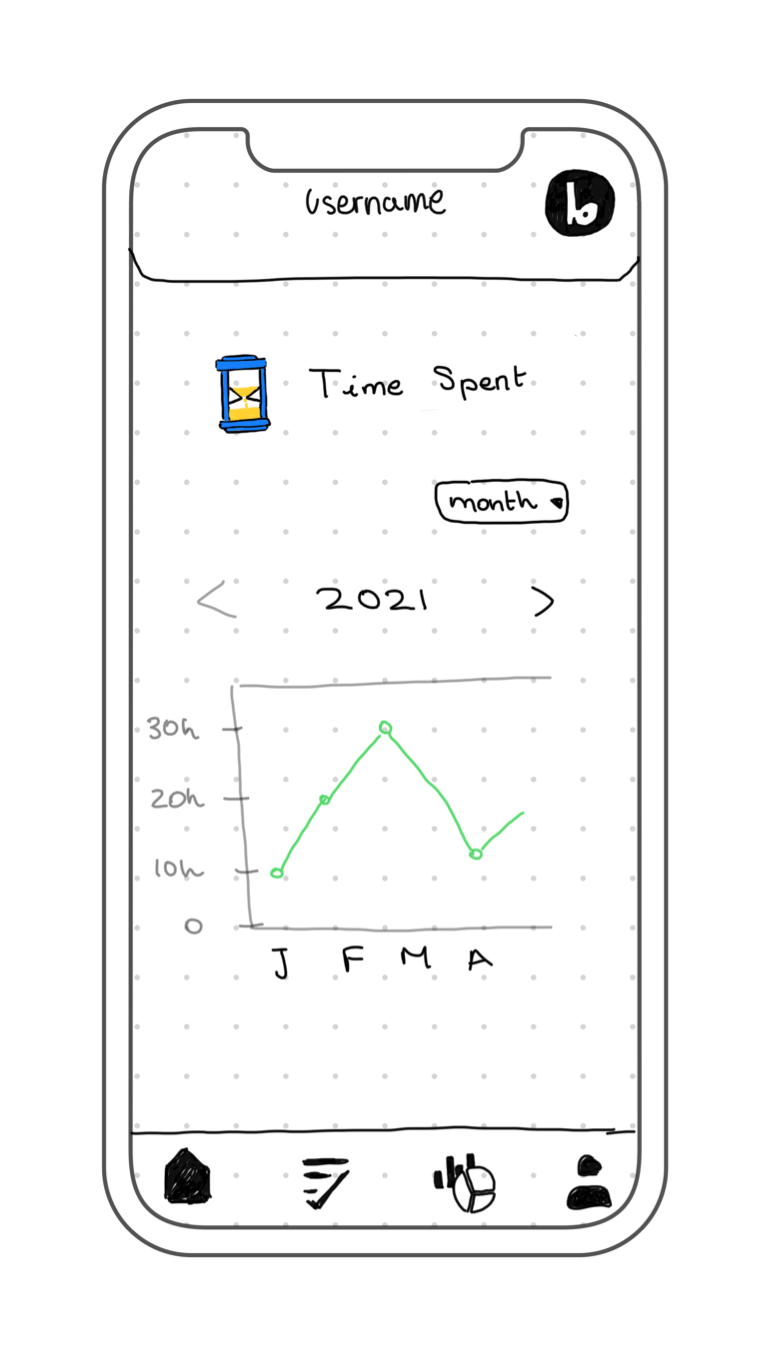
\includegraphics[width=0.72\textwidth]{assets/screens/stats/Stats - 3.png}
        \caption{Stats' detail}
        \label{fig:design_screen_stats_3}
    \end{subfigure}
       \caption{Stats' screens}
       \label{fig:design_screen_stats}
\end{figure}

\subsubsection{User}
This screen allow the user to customize the application and change personal information. \\
\begin{figure}[H]
    \centering
        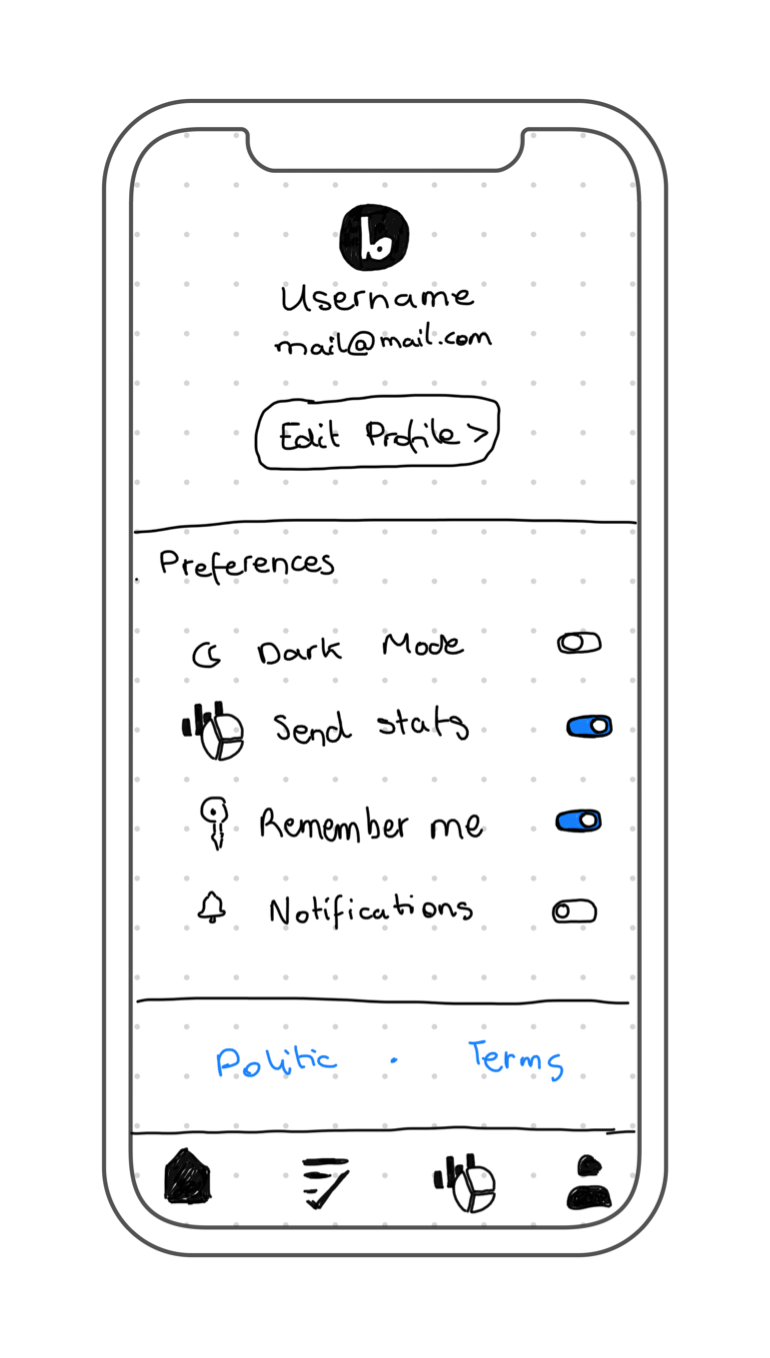
\includegraphics[width=0.24\textwidth]{assets/screens/User.png}
    \caption{User screen}
    \label{fig:design_user}
\end{figure}

\subsubsection{Navigation}
In this figure we can see how a user would interact with every screen and the navigation between all of them. \\

Firstly, there is a first layer that the user has to pass, which is the auth layer. In order to use the rest of the application (private routes), the user \\
should sign in the application. \\

Secondly, there is a row containing the main screens of the application. Using the \textbf{bottom bar} the user is able to move from one to another. \\

Finally, we see all the rest of the subpages of the application, that contains more detailed information or actions. Among them we can see more in-detail stats \\
or doing/reviewing quizes.
If we take a look into the quiz ramification, we see a use case: create a test and do it. The user first customize the quiz, selecting the difficulty, number of questions and type of quiz. Then the user reply to the questions of the quiz itself and then the user is able to see the quiz result.\\

\begin{figure}[H]
    \centering
        \includegraphics[width=\textwidth]{assets/lofi.png}
    \caption{Low-fidelity design}
    \label{fig:design_lofi}
\end{figure}

